\subsection{Builder}
\label{builder}

\textbf{Scopo}: Creazionale \\
\textbf{Raggio d'azione}: Oggetti

\paragraph{Definizione} Il patter Builder permette di separare la costruzione di un oggetto complesso dalla sua rappresentazione, in modo che lo stesso processo di costruzione possa essere utilizzato per creare rappresentazioni diverse.

\paragraph{Motivazione} Prendiamo in considerazione un’applicazione capace di leggere documenti in formato RTF che può supportare la conversione in altri formati (ASCII, LaTeX).

\begin{figure}[H]
    \centering
    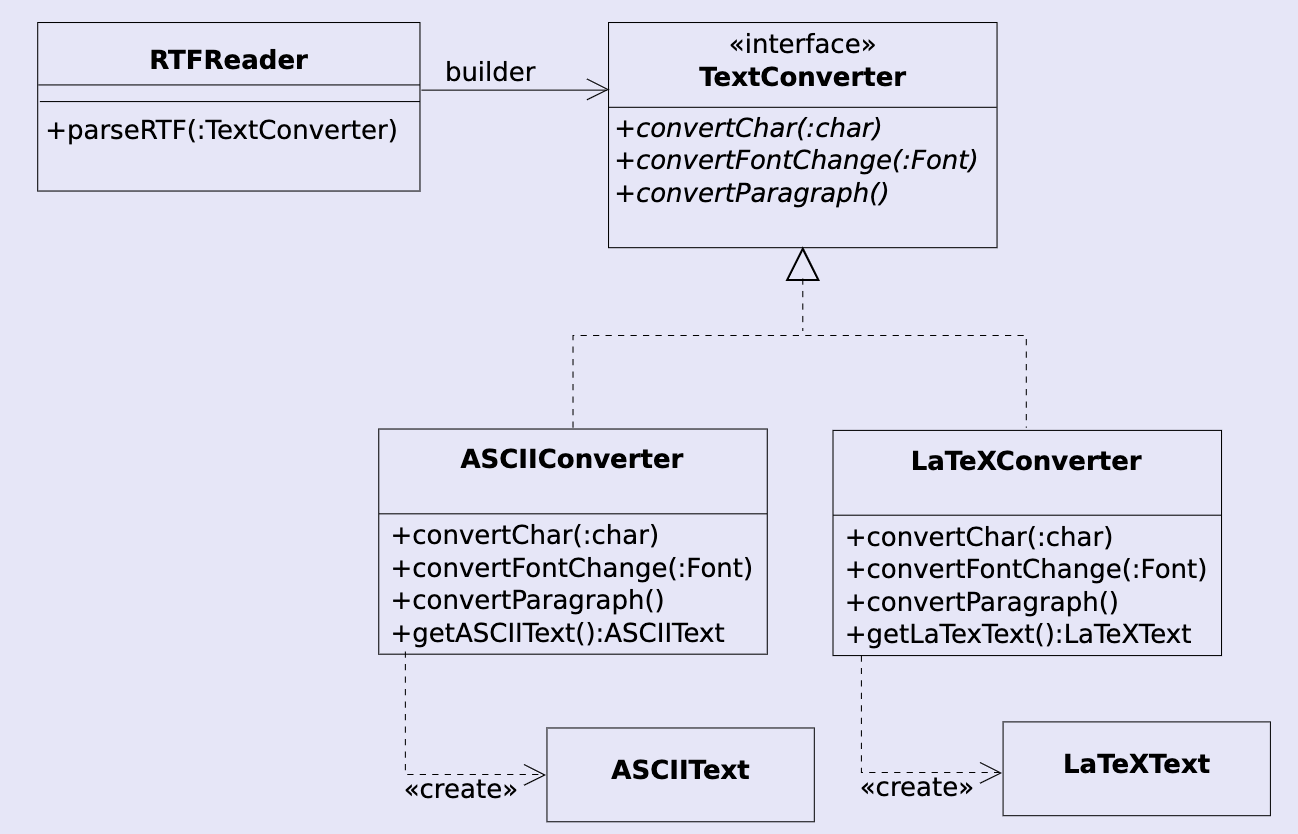
\includegraphics[width=0.75\linewidth]{assets/pattern/builder/builder-esempio.png}
\end{figure}

Una soluzione consiste nel configurare la classe RTFReader con un oggetto conforme all’interfaccia TextConverter in grado di gestire la conversione in un altro formato. Il documento nel formato di uscita viene costruito man mano che gli elementi del documento RTF sono analizzati.

\begin{figure}[H]
    \centering
    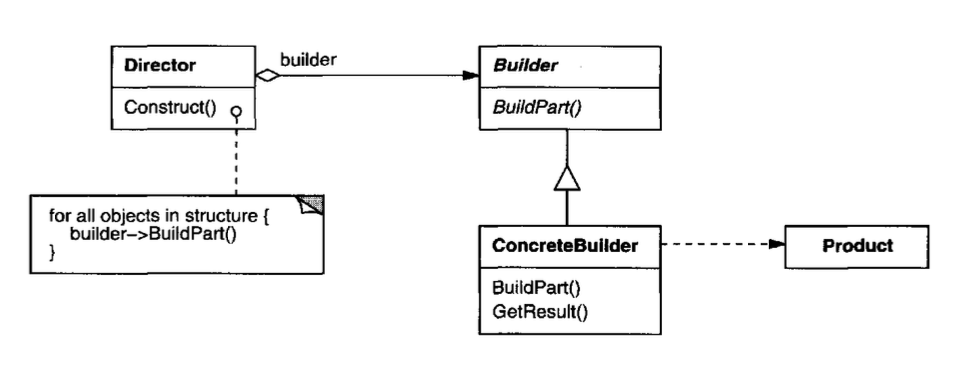
\includegraphics[width=0.75\linewidth]{assets/pattern/builder/builder-struttura.png}
    \caption{Class Diagram del pattern Builder}
\end{figure}

\paragraph{Applicabilità} È consigliabile utilizzare il pattern Builder quando:
\begin{itemize}
    \item L'algoritmo di creazione di un oggetto complesso è indipendente dalle parti che lo costituiscono.
    \item Il processo di costruzione deve permettere rappresentazioni diverse pper l'oggetto costruito.
\end{itemize}

\paragraph{Struttura} Il pattern è composto da:
\begin{itemize}
    \item \textbf{Builder}: specifica l’interfaccia astratta che crea le parti dell’oggetto Product (Alternativa step-by-step ad AbstractFactory \ref{abstract-factory}). 
    \item \textbf{ConcreteBuilder}: costruisce e assembla le parti del prodotto implementando l’interfaccia Builder; definisce e tiene traccia della rappresentazione che crea.
    \item \textbf{Director}: costruisce un oggetto utilizzando l’interfaccia Builder.
    \item \textbf{Product}: rappresenta l’oggetto complesso e include le classi che definiscono le parti che lo compongono, includendo le interfacce per assemblare le parti nel risultato finale. (Spesso il builder è usato per costruire Composite \ref{composite})
\end{itemize}

\begin{figure}[H]
    \centering
    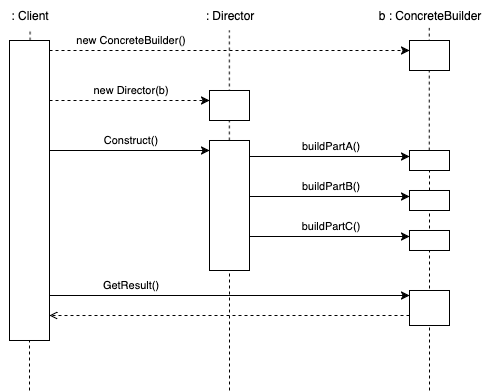
\includegraphics[width=0.75\linewidth]{assets/pattern/builder/builder-sequence.drawio.png}
    \caption{Sequence Diagram del pattern Builder}
\end{figure}

\begin{enumerate}
    \item Il Client create un oggetto Director e lo configura con il Builder desiderato. 
    \item Il Director notifica il Builder quando una parte di un prodotto deve essere costruita.
    \item Il Builder gestisce la richiesta e aggiunge le parti richieste al Product.
    \item Il Client richiede l'oggetto al Builder.
\end{enumerate}

\paragraph{Conseguenze} Il pattern Builder consente quindi di:
\begin{itemize}
    \item \textbf{Variare la rappresentazione interna di un prodotto}: nasconde la rappresentazione e la struttura interna del prodotto. Nasconde anche come il prodotto viene assemblato.
    \item \textbf{Isolare il codice per la costruzione la rappresentazione}: Ogni ConcreteBuilder contiene tutto il codice necessario a creare ed assemblare un particolare tipo di prodotto. Diversi Director possono riusare lo stesso Builder per creare varianti di Product.
    \item \textbf{Avere maggiore controllo del processo di costruzione}: il Builder costruisce iol prodotto step-by-step sotto la supervisione del Director.
    \item \textbf{Risolvere il problema dei \textit{costruttori telescopici}} :si propone come alternativa a tecnologie come JavaBeans.
\end{itemize}



\newpage

\textbf{Esempio Java}

\begin{minted}[
    fontsize=\footnotesize,
    linenos,
]{java}
public class NutritionFacts { 

    private final int servingSize; 
    private final int servings; 
    private final int calories ; 
    private final int fat ; 
    private final int sodium; 
    private final int carbohydrate; 
    
    public static class Builder { 
        // Required parameters 
        private final int servingSize; 
        private final int servings; 
        
        // Optional 
        private int calories = 0; 
        private int fat = 0; 
        private int carbohydrate = 0; 
        private int sodium = 0; 
        
        public Builder( int servingSize, int servings) { 
            this.servingSize = servingSize; 
            this.servings = servings; 
        } 
        
        public Builder calories ( int val ) { 
            calories = val ; return this;
        } 
        
        public Builder fat ( int val ) { 
            fat = val ; 
            return this; 
        } 
        
        public Builder carbohydrate(int val ) {
            carbohydrate = val; 
            return this; 
        } 
        
        public Builder sodium(int val) { 
            sodium = val; 
            return this; 
        } 
        
        public NutritionFacts build () { 
            return new NutritionFacts(this); 
        } 
    }
    
    private NutritionFacts (Builder builder ) { 
        servingSize = builder.servingSize; 
        servings = builder.servings; 
        calories = builder.calories; 
        fat = builder.fat;
        sodium = builder.sodium; 
        carbohydrate = builder.carbohydrate;
    }
}

// Utilizzo:
NutritionFacts cocaCola = new NutritionFacts.Builder(240, 8)
                            .calories(100)
                            .sodium(35)
                            .carbohydrate(27)
                            .build();

\end{minted}


\newpage